\documentclass{iopart}

\usepackage{graphicx}
\usepackage[margin=2cm]{geometry}

\begin{document}

\title{Unibody Frame Notes}

\section{Overview}
The Unibody Frame is the structure on the lower half of the robot that combines the baseplate, motor mounts, and midplate normally found on other robots into a single piece of sheet metal that supports every system on the robot.

\section{Unibody Design}
\subsection{Traditional Designs}
The structure of most SSL robots consists of a three unique parts a baseplate, a motor mount and a midplate where the baseplate is commonly a single piece of sheet metal with mounting holes to attach other components including the motor mounts (which supports the wheels and drive motors) and the midplate (which supports the robot's electronics) are either mounted to the top of the motor mounts or standoffs on the baseplate.

% 4 part figure showing off the thunderbots design
% Removal of the wings

\subsection{Trade-offs of a Unibody Design}
%\subsubsection{Repairability}

%\subsubsection{Cost}
\begin{itemize}
    \item Repairability
    \medskip

    The monolithic nature of the unibody frame means that during competition if the frame gets damaged in some way that can't be fixed we'll need to replace the entire frame rather than swap out just the one motor mount or standoff. This increases the cost to maintain robots and the space needed to store spare parts since the frames can't be stacked compactly.

    \medskip
    \item Cost

    The cost of machining metal parts falls into a hierarchy where parts that can be reduced to a one-dimensional piece of wire are cheaper to make than a part that can only be reduced to two-dimensional piece of sheet metal which itself is cheaper than parts whose design must be three-dimensional. Thunderbots's motor mounts are 3D because of the holes on the bottom for fastening it to the baseplate. The unibody design sits lower on the cost hierarchy. Early quotes from SendCutSend priced completed unibody frames at \$25 each whereas in 2021 motor mounts cost about \$7.50 each which does not include the materials and waterjet time need to make the midplate and baseplate.

    \medskip
    \item Flexibility in Design

    Since the functions of mounting the kicker, motors, midplate, baseplate PCB, etc. are all combined into a single part, future changes to their requirements either need to be accounted for in the specification of the frame or the frame needs to be replaced.

    \medskip
    \item Weight
    
    A traditional design where motor mounts are bolted to a baseplate places a minimum thickness on the parts to have enough material for the screws to thread into. Combining the baseplate and motor mounts into a single part lifts this requirement allowing for thinner and lighter designs.
\end{itemize}

\section{Mounting Holes}
\subsection{Kicker Mounting}
The center of the chassis has two sets of mounting holes, the inner four holes match the hole pattern on the off-the-shelf solenoid bought from Amazon\footnote{amazon.ca/Abletop-Solenoid-Electromagnetic-Electric-Automobiles/dp/B07G15X91N} and the outer four screw clearances are to give the chassis the flexibility to design a new kicker and add it without much modification. The baseplate has a rectangular hole cut in the center to improve the efficiency of the kicker by reducing the material that gets energized when the solenoid is powered. A beam stretches across the rectangular cutout to provide material to mount the front half of the off-the-shelf kicker to. There is an extra gap where the mounting beam meets the edge of the rectangular cutout, this is there because when we upgrade our kicker we will want to cut out that beam and adding this gap means we won't need to put as much effort into making sure we cut and file it flush with the edge of the cutout.

% Probably a good place for more graphics

\subsection{Midplate Mounting}
The midplate as a PCB which rests on the flanges at the top of the motor mounts. There are four holes for mounting the midplate the front two holes are threaded to allow thumbscrews to fasten the midplate, the rear holes are filled with 3D printed studs to help align placement of the midplate and restrict the rotations of the midplate.

\subsection{Baseplate PCB Mounting}
The bottom of the chassis also supports a baseplate PCB that handles power delivery and CAN to the mechanical systems. There are four holes for fastening this PCB to the chassis. One of the rear mounting holes for the PCB uses a threaded post rather than a screw to support a hook that provides strain relief for cables running between the baseplate and the midplate as well as keep them away from the wheels.

\subsection{Breakbeam Housing}
There is a single thread hole in the front of the baseplate for fastening down the breakbeam housing.

\begin{center}
    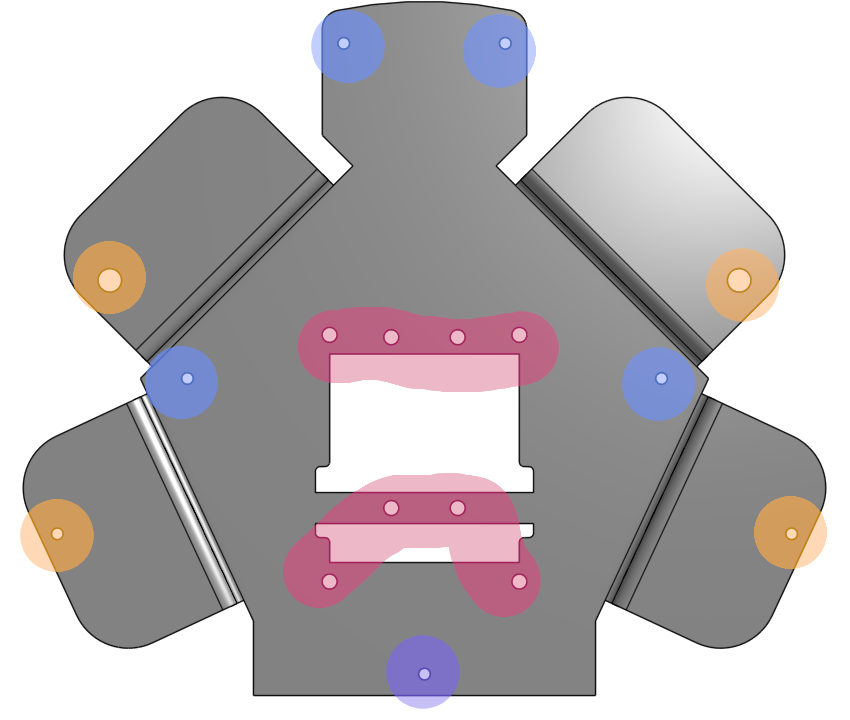
\includegraphics{graphics/mount_holes.png}\\
    Holes highlighted in yellow are for attaching the midplate; blue is for attaching the baseplate PCB; magenta for mounting the kicker where the inner four are for the store bought solenoid and the outer four are for a future kicker; purple is for attaching the breakbeam housing.
\end{center}

\subsection{Simovr Mounting}
The outer four holes on the motor mount are tapped for standoffs that hold the motor drivers.

\subsection{Motor Mounting}
The inner holes are for supporting the motors, the big hole in the center gives room for the motor shaft and the smaller holes are for fastening it to the motor mount.

\begin{center}
    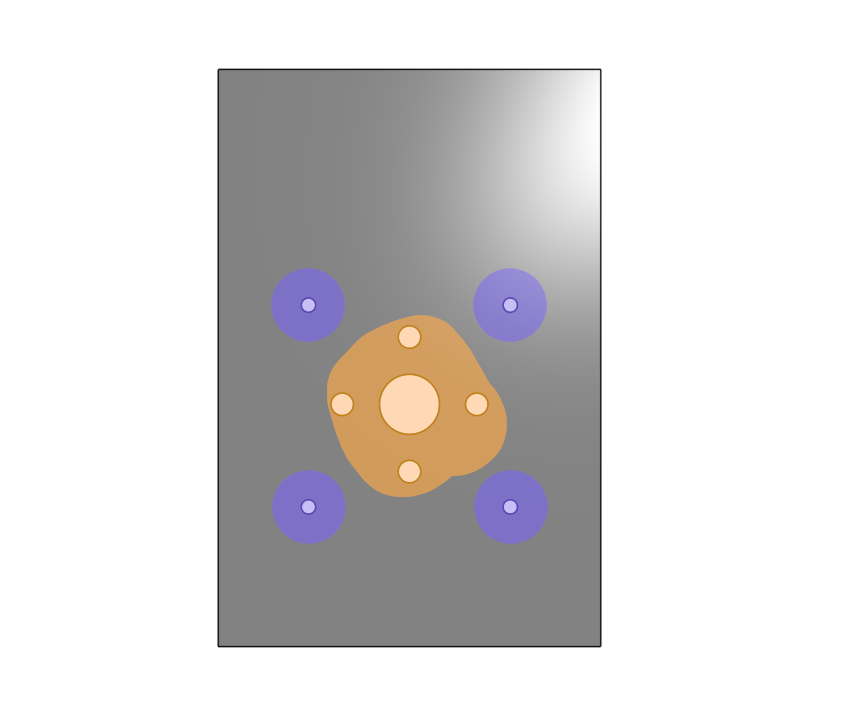
\includegraphics{graphics/motor_mount.png}\\
    Holes highlighted in yellow are for the motor and purple is for the motor dirver.
\end{center}

\section{Material and Thickness Considerations}
The material we ordered for the first iteration of the chassis is 14 gauge thickness aluminum-5052 ordered from SendCutSend.

\subsection{Aluminum vs. Steel}
The two materials we considered for the chassis are aluminum and cold-rolled steel. The pros of each material are:

\begin{center}
    \begin{tabular}{c|c}
        Aluminum & Steel \\
        \hline
        About 65\% lighter & 47\% higher yield strength \\
         & Can spot weld in more material
    \end{tabular}
\end{center}

\subsection{Threading}
Every threaded part except the standoffs for the motor drivers is M3x0.5 if we want these to thread directly into the chassis instead of needing extra hardware such as a nut welded over the holes we want a thickness of at least about 1.5mm so we can have at least 3 threads engaged.

\subsection{Flexural Strength}
In 2019, we measured the maximum acceleration of Thunderbots's robots to be approximately 3.2m/s$^2$ and weighing about 2.7Kg therefore the force that robot could provide is about 8.6N. To gives us a large margin of safety we aimed to calculate the thickness required for the robot to resist a 20N force applied to one of the wheels without yielding. The failure force on a cantilever beam is given by the equation:

\begin{center}
    \begin{equation}
        F_{Fail} = \frac{S_ybh^2}{6L}
        \label{eq:fail_force}
    \end{equation}
\end{center}

Where $S_y$ is the yield strength, $b$ is the width, $h$ is the thickness, $L$ is the length, and $F$ is the force. If we take the length of the beam to be the distance from the bend in the chassis to the motor shaft we get the following values.
\begin{center}
    \begin{tabular}{l|l}
        $S_y$ (Al) & 193 MPa\\
        $S_y$ (steel) & 285 MPa\\
        $b$ & 42 mm \\
        $L$ & 36.24 mm
    \end{tabular}
\end{center}

Solving equation \ref{eq:fail_force} for thickness suggests a minimum thickness of 0.73mm for aluminum and 0.60mm for steel.

\subsection{Impact Resistance}
While we would have liked to calculate how increasing thickness would affect our robot's ability to withstand collisions we were unable to come up with any reasonable estimates. And could not find any methods to estimate how much damage a collision might do in the literature that didn't require already having a prototype.

\section{Errors}
The first batch of chassis we ordered had the wrong hole placement for the motors we have. We corrected this issue by drilling the correct holes at a 45 deg orientation to the existing holes.

\begin{center}
    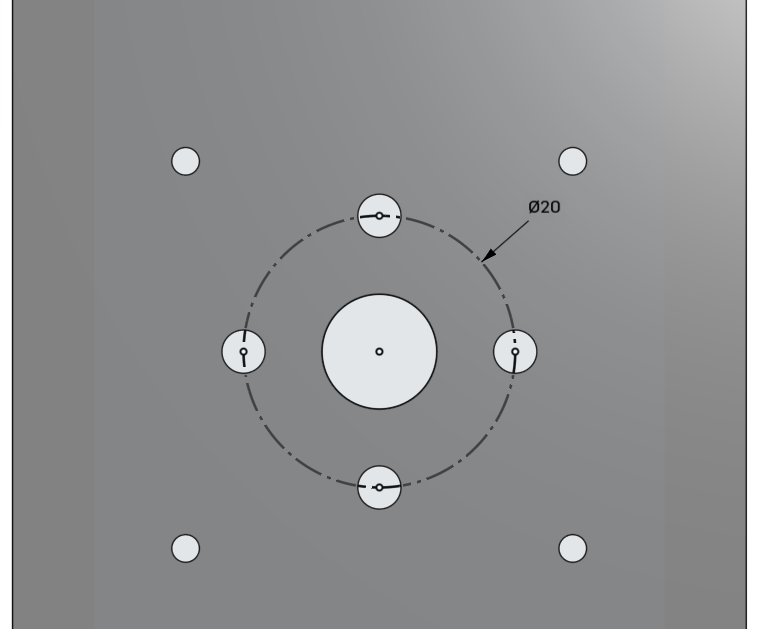
\includegraphics[width=0.4\textwidth]{graphics/wrong_holes.png}
    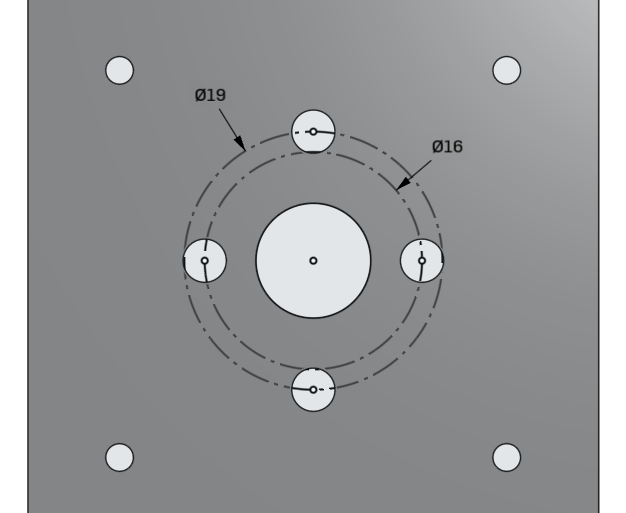
\includegraphics[width=0.4\textwidth]{graphics/right_holes.png}\\
    Left, purchased motor mount hole pattern. Right, the correct hole pattern that matches our motors.
\end{center}

\end{document}